\section{Durchführung}
\label{sec:Durchführung}

Der Lock-In-Verstärker ist gegeben wie in \autoref{fig:f2} dargestellt.
\begin{figure}[H]
    \centering
        \centering
        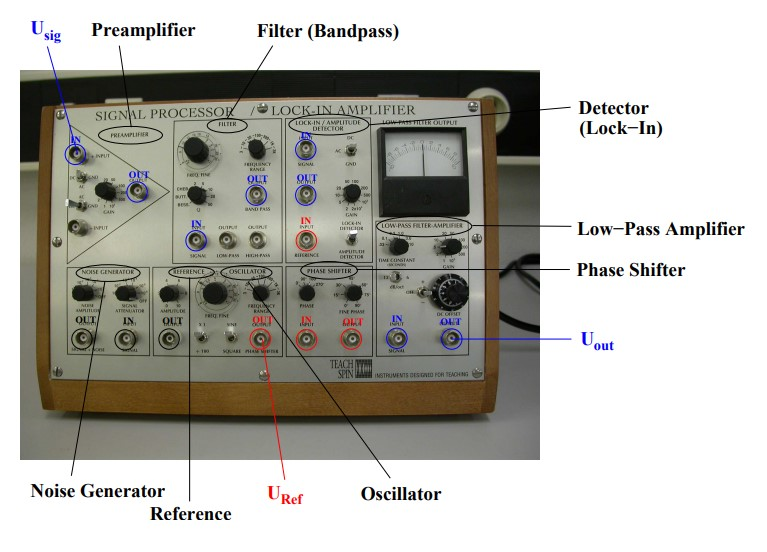
\includegraphics[width=0.95\textwidth]{Bilder/LIV.jpg}
        \caption{Der Lock-In-Verstärker und seine Funktionen. \cite{anleitung2}}
    \hfill
    \label{fig:f2}
\end{figure}
\noindent Zu erkennen ist, dass die Filter, der Phasenschieber, ein
Funktionsgenerator, ein Rauschgenerator, ein TP-Verstärker und ein Amplituden-
und Lock-In-Detektor eingebaut sind. Das Oszilloskop, welches an den Detektor
angeschlossen ist, dokumentiert alle Signale, sodass diese auf dem Display
ausgegeben und skizziert werden.
\par\vspace{0.5em}
\noindent Zunächst wird geprüft, welche Ausgänge die Spannungsamplitude 
beeinflussen und welcher für eine konstante Spannung sorgt.
\par\vspace{0.5em}
\noindent Als nächstes wird die Schaltung aus \autoref{fig:f3} aufgebaut. Dazu
wird der Noise Generator auf $\texttt{OFF}$ gestellt. Ein Signal $U_{sig}$ mit einer
Frequenz von 1 kHZ und 10 mV wird auf den Verstärker gegeben und mit dem 
Referenzsignal $U_{ref}$ gemischt. Die Signale verfügen dabei über eine 
gleiche Frequenz. Die resultierenden Ausgangssignale werden für 5 verschiedene 
Phasen skizziert.
\begin{figure}[H]
    \centering
        \centering
        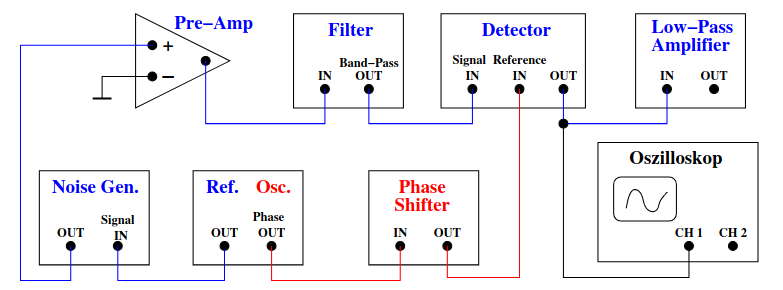
\includegraphics[width=0.9\textwidth]{Bilder/baute1.png}
        \caption{Erster Aufbau. \cite{anleitung2}}
    \hfill
    \label{fig:f3}
\end{figure}
\noindent Anschließend wird ein zusätzliches Rauschsignal via Noise Generator 
hinzugefügt und der vorherige Messvorgang wiederholt. Die dabei entsthenden 
Unterschiede der Signale werden ausgewertet.
\par\vspace{0.5em}
\noindent Zum Schluss wird die Schaltung gemäß \autoref{fig:f4} installiert.
Zusätzlich werden eine Leuchtdiode und eine Photodiode genutzt.
Die Leuchtdiode mit einer Rechteckspannung wird mit einer Frequenz im Bereich 
von 50 bis 500 Hz blinken gelassen. Die Photodiode hingegen misst das ausgesendete 
Licht.
\begin{figure}[H]
    \centering
        \centering
        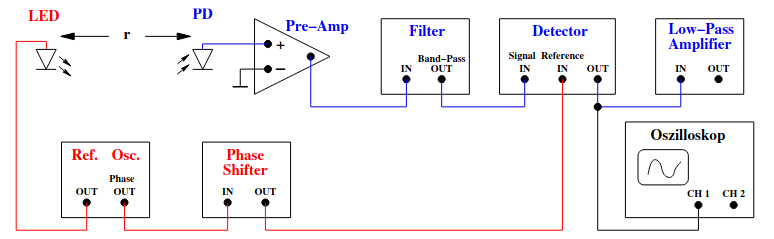
\includegraphics[width=0.9\textwidth]{Bilder/baute2.png}
        \caption{Zweiter Aufbau. \cite{anleitung2}}
    \hfill
    \label{fig:f4}
\end{figure}